\documentclass[10pt,hyperref={colorlinks,linkcolor=black,citecolor=blue!80,urlcolor=blue!60}]{beamer} %"handout" serveix per a treure els \pause
\usepackage[mode=buildnew]{standalone}
\usepackage[utf8]{inputenc}
\usepackage[catalan,english]{babel}
\usepackage{amsmath,amssymb}
\usepackage{tikz}
\usepackage{pgfplots}
\usepackage{graphicx}
\usepackage{subfig}
\usepackage{biblatex}
\usepackage{stmaryrd}
\usepackage{csquotes}
\usepackage{physics}

\usetheme{Copenhagen}
\usecolortheme{seahorse}

\addbibresource{references.bib}

\pgfplotsset{compat=newest}

%%%%%%%% colors %%%%%%%%
\definecolor{lessgreen}{RGB}{0,100,0}
\definecolor{color1}{RGB}{255,158,1}
\definecolor{color2}{RGB}{255,74,1}
\definecolor{color4}{RGB}{180,0,0}
%%%%%%%%%%%%%%%%%%%%%%%%

%%%%%%%%% setbeamer %%%%%%%%%
\setbeamersize{text margin left=0.3cm,text margin right=0.3cm}
\setbeamerfont{footnote}{size=\tiny}
\setbeamertemplate{bibliography item}[text]
%%%%%%%%%%%%%%%%%%%%%%%%%%%%%

%%%%%%%% newtheorems %%%%%%%%
\theoremstyle{definition}
\newtheorem{defin}[theorem]{Definició}
%%%%%%%%%%%%%%%%%%%%%%%%%%%%%

%%%%%%%% newcommands %%%%%%%%
\newcommand\enllas{\raise.5pt\hbox{$\boxempty\kern-4.85pt{}^{\nearrow}$}\kern-2pt}
\DeclareFieldFormat{url}{%
  \ifhyperref
    {\href{#1}{\enllas}}
    {\url{#1}}}% url symbol for references. It is needed \usepackage{stmaryrd}

\newcommand{\0}{\ensuremath{\vb{0}}}
\newcommand{\N}{\ensuremath{\vb{N}}}
\newcommand{\X}{\ensuremath{\vb{X}}}
\newcommand{\Y}{\ensuremath{\vb{Y}}}
\newcommand{\Z}{\ensuremath{\vb{Z}}}
\newcommand{\NN}{\ensuremath{\mathbb{N}}} % set of real numbers
\newcommand{\RR}{\ensuremath{\mathbb{R}}} % set of real numbers
\newcommand\Hz{\text{ Hz}}
\DeclareMathOperator{\diss}{diss}
\DeclareMathOperator{\arccosh}{arccosh}
%%%%%%%%%%%%%%%%%%%%%%%%%%%%%

\institute[UAB]{Taller de modelització\\
\vspace{5pt}Grau en Matemàtiques\\
\vspace{5pt}Universitat Autònoma de Barcelona}
\title[Mesures de dissonància]{Mesures de dissonància}
\author[Víctor, Oriol, Carlo]{Víctor Ballester\and Oriol Bosquet\and Carlo Sala}
\date{Juny 2021}

\begin{document}
\selectlanguage{catalan}
\frame{\titlepage}
\begin{frame}{Objectiu del treball}
    És ben sabut que hi ha combinacions de notes musicals que sonen més bé que d'altres. Des de l'antiguitat se sap que això correspon al fet que certs paràmetres identificatius de les notes són proporcionals a nombres enters senzills.\par\vspace{1cm}
    L'objectiu del treball és donar una modelització matemàtica de com mesurar el grau de dissonància produït quan toquem dues (o més) notes musicals simultàniament.
\end{frame}
\begin{frame}{Definicions prèvies}
    \only<1| handout:1>{\begin{defin}[Dissonància]
        Qualitat de dos o més sons amb una relació de freqüències concreta, que sonen poc agradables a l'oïda humana.
    \end{defin}
    \begin{defin}[Consonància]
        Qualitat de dos o més sons amb una relació de freqüències concreta, que sonen agradables a l'oïda humana.
    \end{defin}}
    \only<2| handout:2>{\begin{defin}[So simple]
        Siguin $f\in(0,\infty)$ i $a\in[0,\infty)$. Anomenem \textit{so simple} o \textit{so pur} el parell $s=(f, a)$ on $s$ és el so sinusoidal d'equació: $$y_s(t)=a\sin(2\pi f)$$ Denotem per $\mathcal{S}$ el conjunt de sons simples.
    \end{defin}
    \begin{defin}[So complex]
        Siguin $s_1,\ldots,s_n\in\mathcal{S}$ són simples tals que $s_i=(f_i,a_i)$ per $i=1,\ldots,n$. Anomenem \textit{so complex} el conjunt $\X=\{s_1,\ldots,s_n\}$ tal que $\X$ és el so d'equació: $$y_{\X}(t)=\sum_{i=1}^ny_{s_i}(t)=\sum_{i=1}^na_i\sin(2\pi f_it)$$ Denotem per $\mathcal{C}$ el conjunt de sons complexos.
    \end{defin}}
\end{frame}
\begin{frame}{Operacions definides sobre $\mathcal{C}$}
    Suposem $\X,\Y\in\mathcal{C}$, on $\X=\{(f_1,a_1),(f_2,a_2),\ldots,(f_n,a_n)\}$.\par\pause
    \begin{defin}
        Definim la suma $\oplus$ entre sons complexos com l'aplicació:
        $$\begin{array}{r@{\hspace{0.5\tabcolsep}}c@{\hspace{0.5\tabcolsep}}c@{\hspace{0.5\tabcolsep}}l}
            \oplus:&\mathcal{C}\times\mathcal{C}&\longrightarrow&\mathcal{C}\\
            &(\X,\Y)&\longmapsto&\X\oplus \Y:=\X\cup\Y
        \end{array}$$
    \end{defin}\pause
    \begin{defin}
        Definim el producte $\cdot$ d'un so complex per un escalar com l'aplicació
        $$\begin{array}{r@{\hspace{0.5\tabcolsep}}c@{\hspace{0.5\tabcolsep}}c@{\hspace{0.5\tabcolsep}}l}
            \cdot:&\mathcal{C}\times[0,\infty)&\longrightarrow&\mathcal{C}\\
            &(\X,\lambda)&\longmapsto&\lambda\cdot \X:=\Z
        \end{array}$$
        on $\Z=\{(f_1,\lambda a_1),(f_2,\lambda a_2),\ldots,(f_n,\lambda a_n)\}\in\mathcal{C}$.
    \end{defin}  
\end{frame}
\begin{frame}{Model per a sons complexos}
    Suposem que tenim una funció $\delta$ de dissonància per a sons simples:
    \begin{align*}
        \delta:\mathcal{S}\times\mathcal{S}&\longrightarrow\RR\\
        (s_1,s_2)&\longmapsto\delta(s_1,s_2)
    \end{align*}
    que satisfà:
    \begin{enumerate}
        \item $\delta(s_1,s_2)=\delta(s_2,s_1)$ $\forall s_1,s_2\in\mathcal{S}$.\pause
        \item $\delta(\lambda\cdot s_1,s_2)=\lambda\delta(s_1,s_2)$ $\forall s_1,s_2\in\mathcal{S}$ i $\forall\lambda\in[0,\infty)$.\pause
        \item $\delta(s_1,\lambda\cdot s_2)=\lambda\delta(s_1,s_2)$ $\forall s_1,s_2\in\mathcal{S}$ i $\forall \lambda\in[0,\infty)$.
    \end{enumerate}
\end{frame}
\begin{frame}
    \begin{defin}
        Definim la funció $d$ de \textit{dissonància relativa} entre $\X=\{s_i\}_{i=1}^n,\Y=\{r_i\}_{i=1}^m\in\mathcal{C}$ com:
    $$d(\X,\Y):=\frac{1}{2}\sum_{i=1}^n\sum_{j=1}^m\delta(s_i,r_j)$$
    \end{defin}\pause
    \begin{alertblock}{Mesura de dissonància de sons complexos}
        Definim la dissonància $D$ d'un so complex $\X$ com: $$D(\X):= d(\X,\X)$$
    \end{alertblock}
    Es pot comprovar que: $$D(\X\oplus\Y)=D(\X)+D(\Y)+2d(\X,\Y)$$\pause O més en general, donats $n$ sons complexos $\X_1,\ldots,\X_n\in\mathcal{C}$ es compleix que:\par
    $$D(\X_1\oplus\cdots\oplus\X_n)=\sum_{i=1}^nD(\X_i)+\sum_{\substack{i,j=1\\i\ne j}}^nd(\X_i,\X_j)=\sum_{i,j=1}^nd(\X_i,\X_j)$$
\end{frame}
\begin{frame}{Teoria auditiva}
    Per tal de crear la funció $\delta$ necessitem fer menció de \textbf{l'amplada de banda crítica}.\pause
    \setcounter{subfigure}{0}
    \begin{figure}
        \centering
        %\captionsetup[subfigure]{labelformat=empty}
        \subfloat[Còclea \href{https://www.pinterest.com/pin/336995984614355654/}{\enllas}]{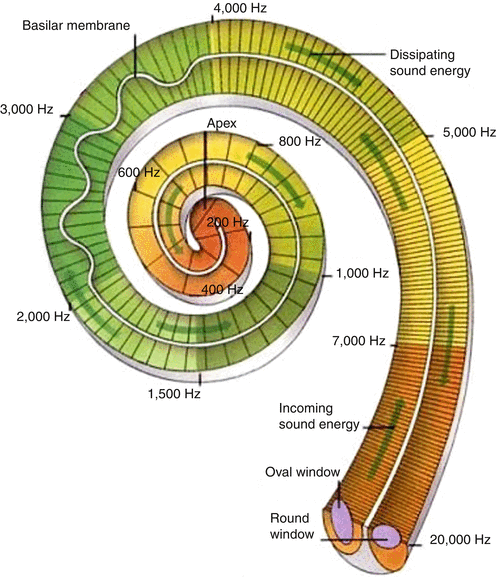
\includegraphics[height=3.2cm]{Imatges_beamer3/coclea.png}}\hspace{1cm}\pause
        \subfloat[Membrana basilar \href{https://www.phys.uconn.edu/~gibson/Notes/Section7_3/Sec7_3.htm}{\enllas}]{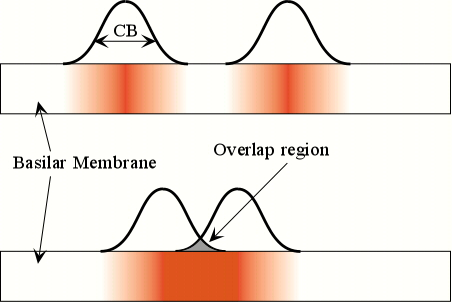
\includegraphics[height=3.2cm]{Imatges_beamer3/basilar_membrane.jpg}}
    \end{figure}\pause 
    \begin{itemize}
        \item Dues freqüències que vibren a la mateixa zona de la membrana basilar són \textbf{dissonants}. \pause
        \item Dues freqüències que no vibren a la mateixa zona de la membrana basilar són \textbf{consonants}. \pause
    \end{itemize}
    Parametrització de l'amplada de banda crítica \cite{hutchinson}:
    \begin{equation*}
        \text{CBW}(f)=1.72 f^{0.65}
    \end{equation*}
    \end{frame}
\begin{frame}{Tria de la funció $\delta$}
    Plomp i Levelt \cite{plomp} van modelitzar empíricament les corbes de dissonància en relació amb la banda crítica.
    \begin{figure}
        \centering
        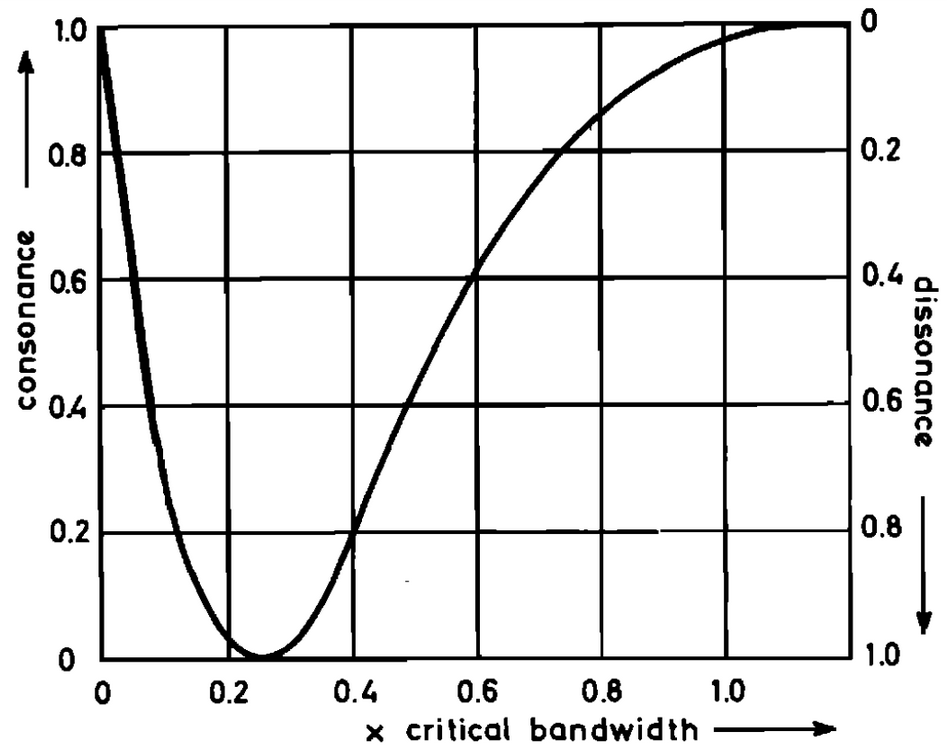
\includegraphics[width=5cm,angle=-0.1]{Imatges_beamer3/plompt-levelt.png}
        \caption{Resultats empírics de Plomp i Levelt \cite{plomp}}
    \end{figure}
    \only<1| handout:0>{\invisible{Algunes equacions que aproximen aquest tipus de funcions són: $$\delta_1(x)=e^{-\alpha x}-e^{-\beta x}\text{ \cite{sethares1}}\qquad\delta_2(x)=e^{-\left(\log(\beta x)\right)^2}\qquad\delta_3(x)=\beta xe^{-\beta x}$$}}
    \only<2| handout:1>{Algunes equacions que aproximen aquest tipus de funcions són: $$\delta_1(x)=e^{-\alpha x}-e^{-\beta x}\text{ \cite{sethares1}}\qquad\delta_2(x)=e^{-\left(\log(\beta x)\right)^2}\qquad\delta_3(x)=\beta xe^{-\beta x}$$}
    \hypersetup{citecolor=black!30}
    \only<3| handout:0>{Algunes equacions que aproximen aquest tipus de funcions són: $$\textcolor{black!20}{\delta_1(x)=e^{-\alpha x}-e^{-\beta x}\text{ \cite{sethares1}}\qquad\delta_2(x)=e^{-\left(\log(\beta x)\right)^2}}\qquad\delta_3(x)=\beta xe^{-\beta x}$$}\hypersetup{citecolor=blue!80}
\end{frame}
\begin{frame}{}
    Considerem dos sons simples $s_1=(f_1,a_1)$ i $s_2=(f_2,a_2)$:\pause
    $$\delta(x)\implies\delta((f_1,a_1),(f_2,a_2))$$\par\pause\vspace{-0.1cm}
    Imposant:
    \begin{enumerate}
        \item $\delta(s_1,s_2)=\delta(s_2,s_1)$\pause
        \item $\max\delta((f_1,1),(f_2,1))=1$ i que s'assoleixi quan $\frac{|f_1-f_2|}{\text{CBW}(f_m)}=0.25$, on $f_m=\frac{f_1+f_2}{2}$\pause
        \item $\delta((f_1,a_1),(f_2,a_2))\propto a_1a_2$\pause
    \end{enumerate}
    Resulta:
    \begin{equation*}
        \delta((f_1,a_1),(f_2,a_2))=a_1a_2\frac{|f_2-f_1|}{\text{CBW}(f_m)\cdot 0.25}e^{1-\frac{|f_2-f_1|}{\text{CBW}(f_m)\cdot 0.25}}
    \end{equation*}\vspace{-0.2cm}
    \begin{figure}
        \centering
        \includestandalone[mode=image|tex,width=5.25cm]{Imatges_beamer3/model2}
    \end{figure}
\end{frame}
\begin{frame}
    Considerem dues notes musicals $\N_1$ i $\N_2$ (amb 9 harmònics) de la forma: $$\N_i=\left\{(f_i,1),\left(2f_i,\frac{1}{2^\alpha}\right),\ldots,\left(7f_i,\frac{1}{7^\alpha}\right)\right\}\quad\text{ per }i=1,2,$$ suposant $a_k=\frac{1}{k^\alpha}$ amb $\alpha=0.75$:\pause
    \begin{figure}
        \centering
        \includestandalone[mode=image|tex,width=9cm]{Imatges_beamer3/complex2}
    \end{figure}
\end{frame}
\begin{frame}{Verificació del model}
    Per tal de verificar el nostre model vam dur a terme un test. \pause
    \begin{itemize}
        \item Cada persona valorava el seu nivell musical (molt baix, baix, intermedi, alt o molt alt).\pause
        \item Hi havia 11 combinacions de dues notes musicals (tocades amb piano).\pause
        \item S'havia de qualificar cada so d'1 (molt dissonant) a 10 (molt consonant).
    \end{itemize}\pause
    En total vam aconseguir 190 respostes.
    \begin{figure}
        \centering
        \includegraphics[width=5.45cm]{Imatges_main/mediana.tex}
    \end{figure}
\end{frame}
\begin{frame}{Conclusions i refinaments}
    Possibles millores:\pause
    \begin{itemize}
        \item Estudiar una possible estructura d'espai vectorial darrere el conjunt de sons complexos\pause
        \item Realitzar el test amb sons de diversos tipus d'instruments (de vent, de corda o de percussió)\pause
        \item Millorar la fiabilitat del test
    \end{itemize}
\end{frame}
\begin{frame}[noframenumbering]{Referències}
    \printbibliography[heading=none]
\end{frame}
\end{document}